\documentclass{llncs}

\usepackage[italian]{babel}
\usepackage[utf8]{inputenc}
% \usepackage{hyperref}
\usepackage{graphicx}

\usepackage[T1]{fontenc}
\usepackage{subcaption}
\captionsetup{compatibility=false}
%\usepackage{float}
\usepackage{amssymb}
\author{Giuseppe De Palma}

\title{Progetto Elaborazione Linguaggio Naturale: Tecniche di Clustering}
\institute{Alma Mater Studiorum - Università di Bologna \\
	\email{giuseppe.depalma@studio.unibo.it}\\
	\email{Matricola: 854846}
}

\newcommand{\acapo}{\vspace{0.5\baselineskip}\\}

\begin{document}
    \maketitle
	
	\begin{abstract}
		Ciaone
	\end{abstract}
	   
	\section{Introduzione}
	Il \textit{clustering} (o analisi dei gruppi) è una forma di \textit{machine learning} non supervisionato che permette di raggruppare in \textit{cluster} elementi non annotati
	dati in input. Un cluster è una collezione di oggetti ``simili'' tra loro che sono ``dissimili'' rispetto agli oggetti degli altri cluster. Questo tipo di machine learning è
	ottimo per partizionare un insieme di dati in diverse ``categorie'', quindi poter eseguire diverse analisi ed ottenere nuove informazioni.
	Applicazioni tipiche in cui il clustering viene molto usato è il riconoscimento di email di spam (le email a scopi pubblicitari o di frode), oppure per l'aggregazione di notizie (Google News ne è un esempio).
	\acapo
	Il clustering trova possibili applicazioni anche nel campo dell'elaborazione del linguaggio naturale. Oltre alle nuove possibili analisi
	sui corpora ed al fornire una visualizzazione pittografica delle parole raggrupate, un interessante utilizzo è quello della \textbf{generalizzazione} delle parole.
	\acapo 
	Possiamo considerare i vari cluster delle classi di equivalenza. Per questo motivo, se avessimo un dataset su cui comporre i cluster fatto di frasi e parole, allora si potrebbe assumere che una
	qualche parola che compare in una frase può essere sostituita con un'altra dello stesso cluster lasciando intatta la correttezza della frase. 
	Ad esempio, se avessimo nel nostro dataset ``per Lunedì'', ``per Martedì'', ``per Mercoledì'', ``per Sabato'', ``per Domenica'', senza avere ``per Giovedì'' e ``per Vernedì'', e avessimo un cluster in cui 
	i giorni della settimana sono raggruppati insieme, allora potremmo generalizzare l'utilizzo della preposizione ``per'' con Giovedì e Vernedì.
	\acapo
	Il clustering, quindi, può essere molto utile anche nell'elaborazione del linguaggio naturale. Nel progetto in studio vengono testate le capacità di alcune tecniche di clustering
	da cui si derivano dei risultati per mostrarne le differenze, i pregi e i difetti. I dati utilizzati negli esperimenti, comunque, non sono parti di testo, ma semplici dataset di vettori numerici 2D in modo tale da poter facilmente 
	visualizzare i grafici relativi ai cluster e determinare le caratteristiche di ogni tecnica.
	\subsection{Outline}
	[\textbf{SCRIVERE OUTLINE}]
	\section{Clustering}
	Ci sono numerosi algoritmi per effettuare clustering, ma essi sono classificabili in poche tipologie: il clustering gerarchico e il clustering partizionale.
	Clustering partizionale consiste nell'ottenere dei cluster, di solito in modo iterativo, ma spesso senza determinare una vera relazione tra gli elementi. Si inizia con un insieme di cluster iniziale ed iterativamente
	si riassegnano gli oggetti nei giusti cluster. Il clustering gerarchico, invece, forma un albero (la gerarchia) degli elementi dove un nodo rappresenta un sotto-cluster del nodo padre e le foglie sono i singoli
	oggetti.
	\acapo
	Un'altra importante distinzione tra gli algoritmi di clustering è il \textit{soft clustering} e \textit{hard clustering}. Nel primo caso, ogni oggetto può essere assegnato a più cluster secondo un qualche
	grado di appartenenza, mentre nel secondo caso ogni oggetto è assegnato ad un unico cluster. In questo progetto vedremo quattro diversi algoritmi, due della classe di clustering gerarchico, due del clustering partizionale.
	I primi tre eseguono hard clustering mentre l'ultimo soft clustering.
	\acapo
	Di seguito sono elencati i metodi implementati e testati:
	\begin{itemize}
		\item Clustering \textbf{gerarchico}
		\begin{enumerate}
			\item Aggregativo
			\item Divisivo
		\end{enumerate}

		\item Clustering \textbf{partizionale}
		\begin{enumerate}
			\item K-Means
			\item EM (soft clustering)
		\end{enumerate}
	\end{itemize}
	
	\subsection{Gerarchico}
	Andando più in dettaglio sulle diverse tecniche, abbiamo detto che la prima classe di clustering permette di creare degli alberi con i cluster e sotto-cluster. 
	Questo può essere ottenuto con un approcco \textit{bottom-up} che è il clustering \textbf{aggregativo},
	il quale inizia dai singoli oggetti e ne raggruppa i più simili, per poi raggruppare i gruppi più simili e così via, fino ad ottenere un unico gruppo
	che sarà la radice dell'albero. Un altro approccio è quello \textit{top-down}, il clustering \textbf{divisivo}, che in modo inverso dal precedente parte 
	dal gruppo comprendente tutti gli elementi e lo divide in sotto-gruppi in modo da massimizzare la similarità intrinseca dei gruppi, 
	fino ad arrivare ai singoli elementi.
	\acapo
	L'albero che si ottiene può essere visualizzato tramite un dendrogramma, come nella figura \ref{ex:dendrogram}.
	Questo diagramma ci mostra le relazioni gerarchiche tra gli oggetti, infatti il suo principale utilizzo è quello di 
	mostrare il modo migliore di organizzare i cluster. 
	\clearpage
	\begin{figure}[h]
		\centering
		\begin{subfigure}[b]{\textwidth}
		   	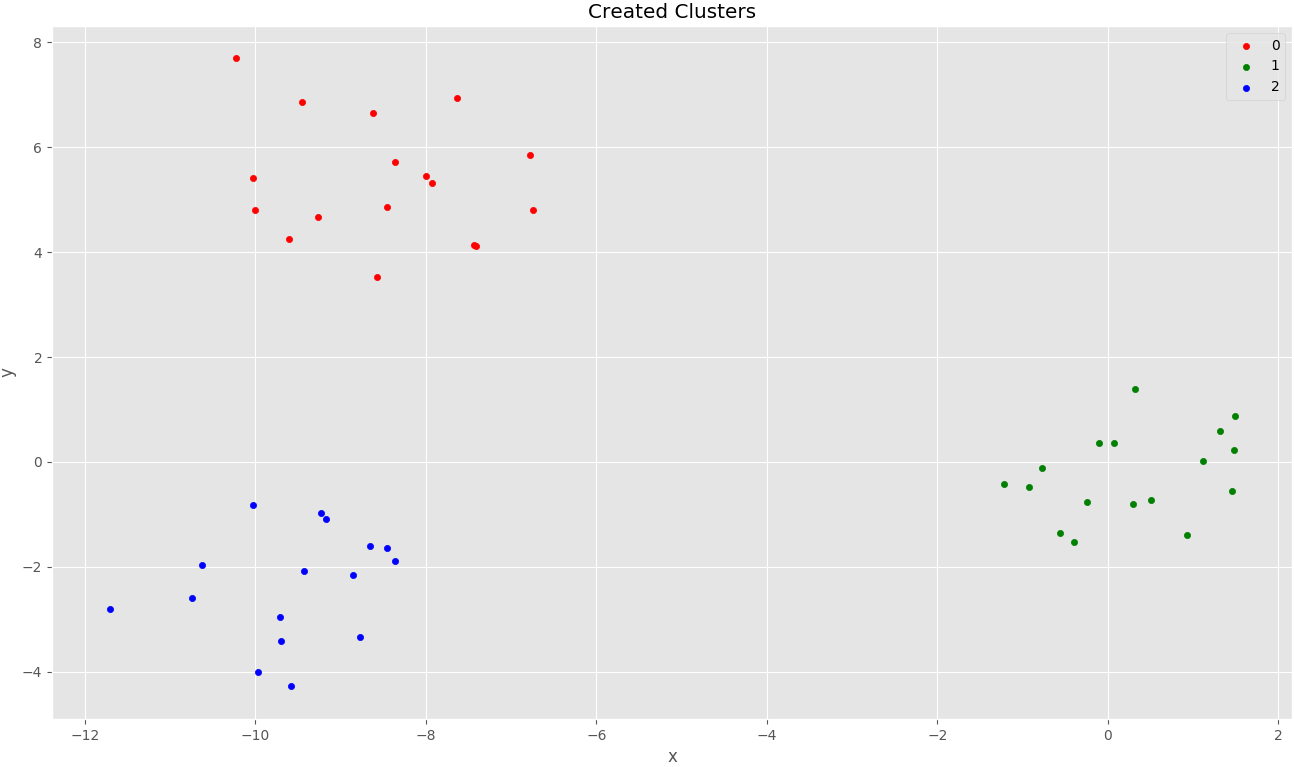
\includegraphics[width=\linewidth]{immagini/created_cluster_dend_ex.png}
		   	\label{fig:1} 
		\end{subfigure}
		
		\begin{subfigure}[b]{\textwidth}
			\centering
		   	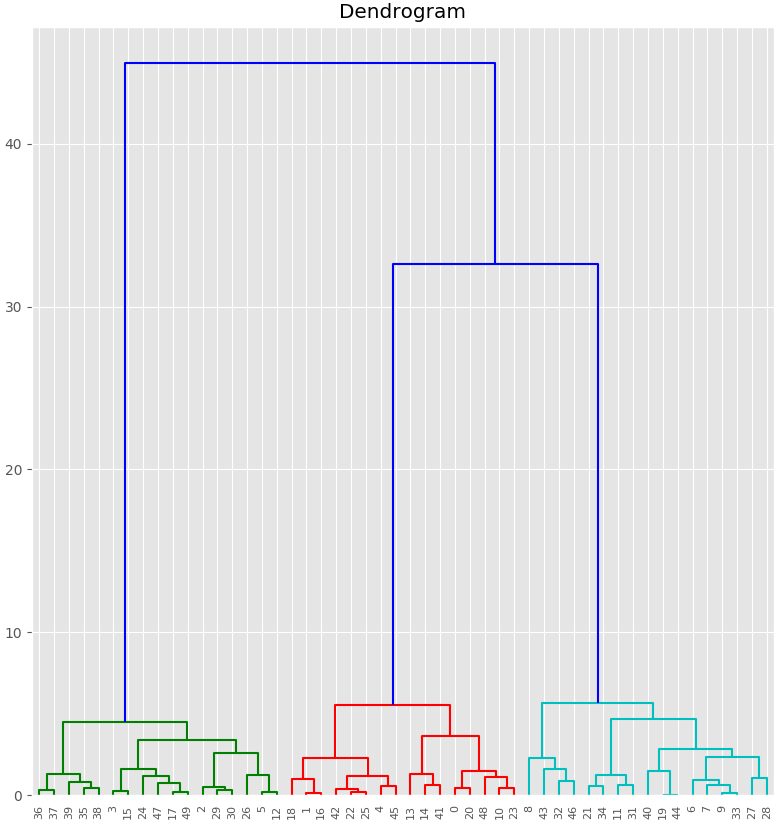
\includegraphics[scale=0.5]{immagini/dendrogam_example.png}
		   	\label{fig:2}
		\end{subfigure}
		
		\caption{(a) insieme di 50 punti pre-divisi in 3 gruppi distinti, su cui si applica il clustering agglomerativo con la funzione di 
		similarità ``ward''. Se ne ricava un dendogramma, in (b), che mostra le relazioni di quei dati. Si noti come tagliando orizzontalmente il cluster per le linee verticali più alte dove non appaiono linee orizzontali, rimangono proprio 3 sotto-cluster.}
		\label{ex:dendrogram}
	\end{figure}
	\clearpage
	Concentrandosi sulle linee verticali, possiamo capire il numero ottimale di cluster
	da prefissare siccome l'asse $y$ misura la somiglianza dei cluster, mentre l'asse $x$ rappresenta gli oggetti e i cluster.
	Disegnando una linea orizzontale che ``taglia'' il dendrogramma, si afferma che i sotto-cluster al di sotto di questa linea saranno i raggruppamenti finali.
	Poichè linee verticali corte rappresentano gradi di similarità più alti tra gruppi, tagliando il dendrogramma per le linee verticali più alte che sono libere da 
	linee orizzontali (quando c'è una unione di cluster), si ha il numero di cluster ottimale a cui assegnare gli elementi,

	\subsubsection{Aggregativo}
	Questo tipo di clustering è realizzato tramite un algoritmo \textit{greedy} che prende in input un insieme di dati $S$, da cui ogni oggetto è considerato essere un piccolo cluster da un elemento.
	Ad ogni passo l'algoritmo determina i due cluster più simili e li unisce in un nuovo cluster. L'algoritmo termina
	quando il cluster contenente tutti gli elementi di $S$ viene formato, il quale sarà l'unico cluster rimanente.
	I modi in cui si possono determinare la similarità dei cluster sono molteplici. L'algoritmo fa uso di una funzione di similarità per calcolare quanto dei cluster sono simili tra di loro, ce ne sono
	diverse, ad esempio alcune molto utilizzate sono:
	\begin{itemize}
		\item single link: ottiene la similarità di due membri \textbf{più} simili da due cluster diversi, rispettivamente;
		\item complete link: ottiene la similarità dei due membri \textbf{meno} simili da due cluster diversi, rispettivamente;
		\item group-average: ottiene la similarità media tra i membri di due cluster.
		\item ward: \textbf{SPIEGARE}
	\end{itemize}
	Nonostante le funzioni di similarità possano differire anche ampiamente, una proprietà che tutte devono avere è la monotonia. Per un insieme di dati $S$ e una funzione di similarità $sim$:
	\begin{center}
		$\forall c, c', \hat{c} \subseteq S$. $min(sim(c, c’), sim(c, \hat{c})) \ge sim(c, c’ \cup \hat{c})$
	\end{center}
	Questo perché l'operazione di unione garantisce	di non aumentare la similarità, quindi una funzione che non obbedisce a questa condizione
	rovinerebbe la gerarchia in quanto cluster non simili, piazzati in parti lontane nell'albero, potrebbero
	ritrovarsi ad essere simili in unioni successive e perciò l'essere vicini nell'albero non corrisponderebbe più al concetto di similarità.

	\subsubsection{Divisivo}
	Come per la controparte aggregativa, dietro il clustering divisivo c'è un algoritmo greedy. Invece di iniziare dai singoli elementi, si inizia dal cluster contenente tutti gli oggetti. Ad ogni iterazione
	si determina quale cluster è quello \textbf{meno} coerente e lo si divide in due. Come prima si utilizzano funzioni di similarità poichè due cluster con oggetti simili sono più coerenti
	di cluster con oggetti non simili. Ad esempio, un cluster con molti oggetti identici ha una coerenza massimale. L'operazione di divisione di un cluster è anch'essa una operazione di clustering, poichè bisogna trovare
	due sotto-cluster. Qualsiasi tecnica di clustering può essere usata per la divisione, anche il clustering aggregativo. Per queste ragione il clustering divisivo è solitamente meno usato.
	However, there are tasks for which top-down clustering is the more nat-
	
	\subsection{Partizionale}
	Diversamente dal clustering appena discusso, gli algoritmi per quello partizionale spesso
	iniziano con una divisione casuale del dataset in vari cluster per poi raffinarli passo dopo passo attraverso 
	la ricollocazione degli oggetti. Da questo procedimento varie domande sorgono. 
	\begin{enumerate}
		\item Quando fermarsi con la ricollocazione?
		\item In quanti cluster dividere il dataset?
		\item In che modo si seleziona il miglior cluster in cui ricollocare un elemento?
	\end{enumerate} 
	Quando fermarsi può essere determinato tramite una metrica sulla qualità dei cluster. Questa può essere una funzione 
	di similarità come la group-average e finchè il risualto incrementa di molto si continua la procedura.
	\acapo
	La stessa metrica può essere utilizzata per rispondere alla seconda domanda. In alcuni casi possiamo già avere
	delle informazioni sul corretto numero di cluster da creare, oppure decidiamo arbitrariamente in quanti cluster dividere il dataset.
	In altri casi invece, possiamo dividere i dati in $k$ cluster osservando l'andamento della metrica.
	Per capire un buon numero di cluster da avere bisogna vedere in quale transizione c'è un 
	incremento sostanziale da $k-1$ a $k$ cluster e un piccolo incremento da $k$ a $k+1$ cluster.
	Trovando un numero $k$ di cluster che abbia questa proprietà, possiamo avere in modo automatico una buona partizione del dataset.
	\acapo
	Per l'ultima questione, sono gli algoritmi per il clustering partizionale che si occupano di come ricollocare gli oggetti, che ora verranno 
	presentati.
	\subsubsection{K-Means}
	K-Means è un algoritmo di hard clustering che definisce i cluster attraverso i loro punti centrali.
	Partendo da dei centroidi iniziali, iterativamente si assegna ogni oggetto al cluster il cui centroide è
	il più vicino, calcolato tramite la distanza euclidea. Una volta che tutti gli elementi sono stati assegnati, si ricalcolano i punti centrali di tutti
	i cluster e si ripete il procedimento di assegnazione così da raffinare il clustering.

	\subsubsection{EM}
	L'algoritmo EM (Expectation-Maximization) è definibile come la versione di K-Means per il soft clustering.
	In quest'algoritmo possiamo vedere ogni cluster come una distribuzione di probabilità (in questo progetto vedremo l'algoritmo EM con \textit{Gaussian mixture model}).
	L'idea è quindi di alternare due step: l'Expectation step dove accade il calcolo delle probabilità per ogni oggetto di essere stato generato da ognuna delle distribuzioni 
	(in K-Means questo è analogo ad assegnare ogni punto ad un cluster). 
	Successivamente c'è il Maximization step, in cui si massimizzano i parametri delle distribuzioni e degli oggetti (pesi, covarianza, medie) così da poter ripetere il primo step. 
	L'equivalente in K-Means è muovere i punti centrali dei cluster per poi procedere con un'altra riallocazione.

	\section{Sessione Sperimentale}
	In questa sezione verranno mostrati vari esperimenti per sottolineare le differenze tra i quattro metodi presentati. Sono stati effettuati diversi test usando diversi dataset di vettori 2D, così da 
	facilmente visualizzare i risultati con grafici. Per l'algoritmo di clustering agglomerativo è stato scelto di usare la funzione di similarità ``ward'', spiegata in precendeza. Per il clustering
	divisivo viene usato K-Means per creare 2 cluster a partire da un cluster più grande, che è lo step di divisione. Per scegliere quale cluster dividere, sono state vagliate diverse possibilità:
	
	\begin{itemize}
		\item Un approccio comune è quello di selezionare il cluster con la massima cardinalità. Questo dà priorità alla produzione di cluster bilanciati rispetto alle dimensioni;
	
		\item Un altro modo è calcolare il raggio di ogni cluster, il quale è la massima distanza tra i punti e il centroide. Quindi si seleziona il cluster con il raggio maggiore;
			
		\item Un altro approccio è calcolare il diametro di ogni cluster, il quale è la massima distanza tra ogni coppia di punti di un cluster.
			Come prima, si va a scegliere il cluster che ha il diametro maggiore.
	\end{itemize}
	
	Data la sua immediatezza, si è scelto di utilizzare il primo approccio.
	\acapo
	Vengono ora mostrati 2 test che rappresentano i diversi esperimenti eseguiti. Nella prima sessione sono stati creati diversi dataset (di cui se ne mostrano 2), dove il clustering 
	agglomerativo e divisivo sono stati adoperati. In seguito con gli stessi dataset, i soggetti saranno i due metodi di clustering partizionale di cui abbiamo parlato. Infine sarà dato un quadro
	generale delle differenze riscontrate.

	\subsection{Agglomerativo vs Divisivo}
	\subsection{K-Means vs EM}
	\subsection{Risultati}

	\section{Conclusioni}

% 	Hierarchical clustering:
% Preferable for detailed data analysis
% Provides more information than
% flat clustering
% No single best algorithm (each of
% the algorithms we describe has
% been found to be optimal for
% some application)
% Less efficient than flat clustering
% (for n objects, one minimally has
% to compute an n x n matrix of
% similarity coefficients, and then
% update this matrix as one pro-
% ceeds)
% Table 14.1 A summary of the attributes
% Non-hierarchical clustering:
% Preferable if efficiency is a con-
% sideration or data sets are very
% large
% K-means is the conceptually sim-
% plest method and should proba-
% bly be used first on a new data
% set because its results are often
% sufficient
% K-means assumes a simple Eucli-
% dean representation space, and
% so cannot be used for many data
% sets, for example, nominal data
% like colors
% In such cases, the EM algorithm
% is the method of choice. It can ac-
% commodate definition of clusters
% and allocation of objects based
% on complex probabilistic models.
% of different clustering algorithms.
    
\end{document}